% !TeX root = Microwave.tex
\chapter{习题}
\section{作业2-3}
\begin{center}
    姓名:韩玉千\hspace{4cm}学号:19020100423
\end{center}

    \paragraph{1}矩形波导$a\times b=22.86\times 10.16\,\si{\square\milli\metre}$,求主模 TE{\scriptsize 10}模的可能工作频率范围。
    \\{\bfseries 解:}\\
    根据 TE{\scriptsize 10}模的截止特性:
    \begin{equation*}
        \beta^2=k^2-k_c^2=(\frac{2\pi}{\lambda})^2-(\frac{\pi}{a})^2>0
    \end{equation*}
    因此
    \begin{equation}
        \lambda<2a\label{Equ: Cut-off Characteristics of TE10}
    \end{equation}
    矩形波导在传输主模时,要求第二模TE{\scriptsize 20}模为凋落模。因此有单模传输条件:
    \begin{equation}
        \lambda>\lambda_{c20}=\frac{2}{\sqrt{(\frac{2}{a})^2+(\frac{0}{b})^2}}=a\label{Equ: Sigle Mode Condition}
    \end{equation}
    结合式(\ref{Equ: Cut-off Characteristics of TE10})和(\ref{Equ: Sigle Mode Condition}),则波长应满足:
    \begin{equation*}
        \lambda\in(a,2a)
    \end{equation*}
    对应工作频率:
    \begin{equation*}
        f\in\left(\frac{c}{2a},\frac{c}{a}\right)
    \end{equation*}
    \rightline{where $c=\SI{3e8}{\metre\per\second}\qquad$}
    得
    \begin{equation*}
        \SI{6.56}{\giga\hertz} < f < \SI{13.12}{\giga\hertz}
    \end{equation*}

    \paragraph{2}画出 TE{\scriptsize 10}模电磁场$E_y, H_x, H_z$的具体场型图。
    \\{\bfseries 解:}如图\ref{Fig: 2-3(2)}所示。\\
    \begin{figure}[htp]
        \centering
        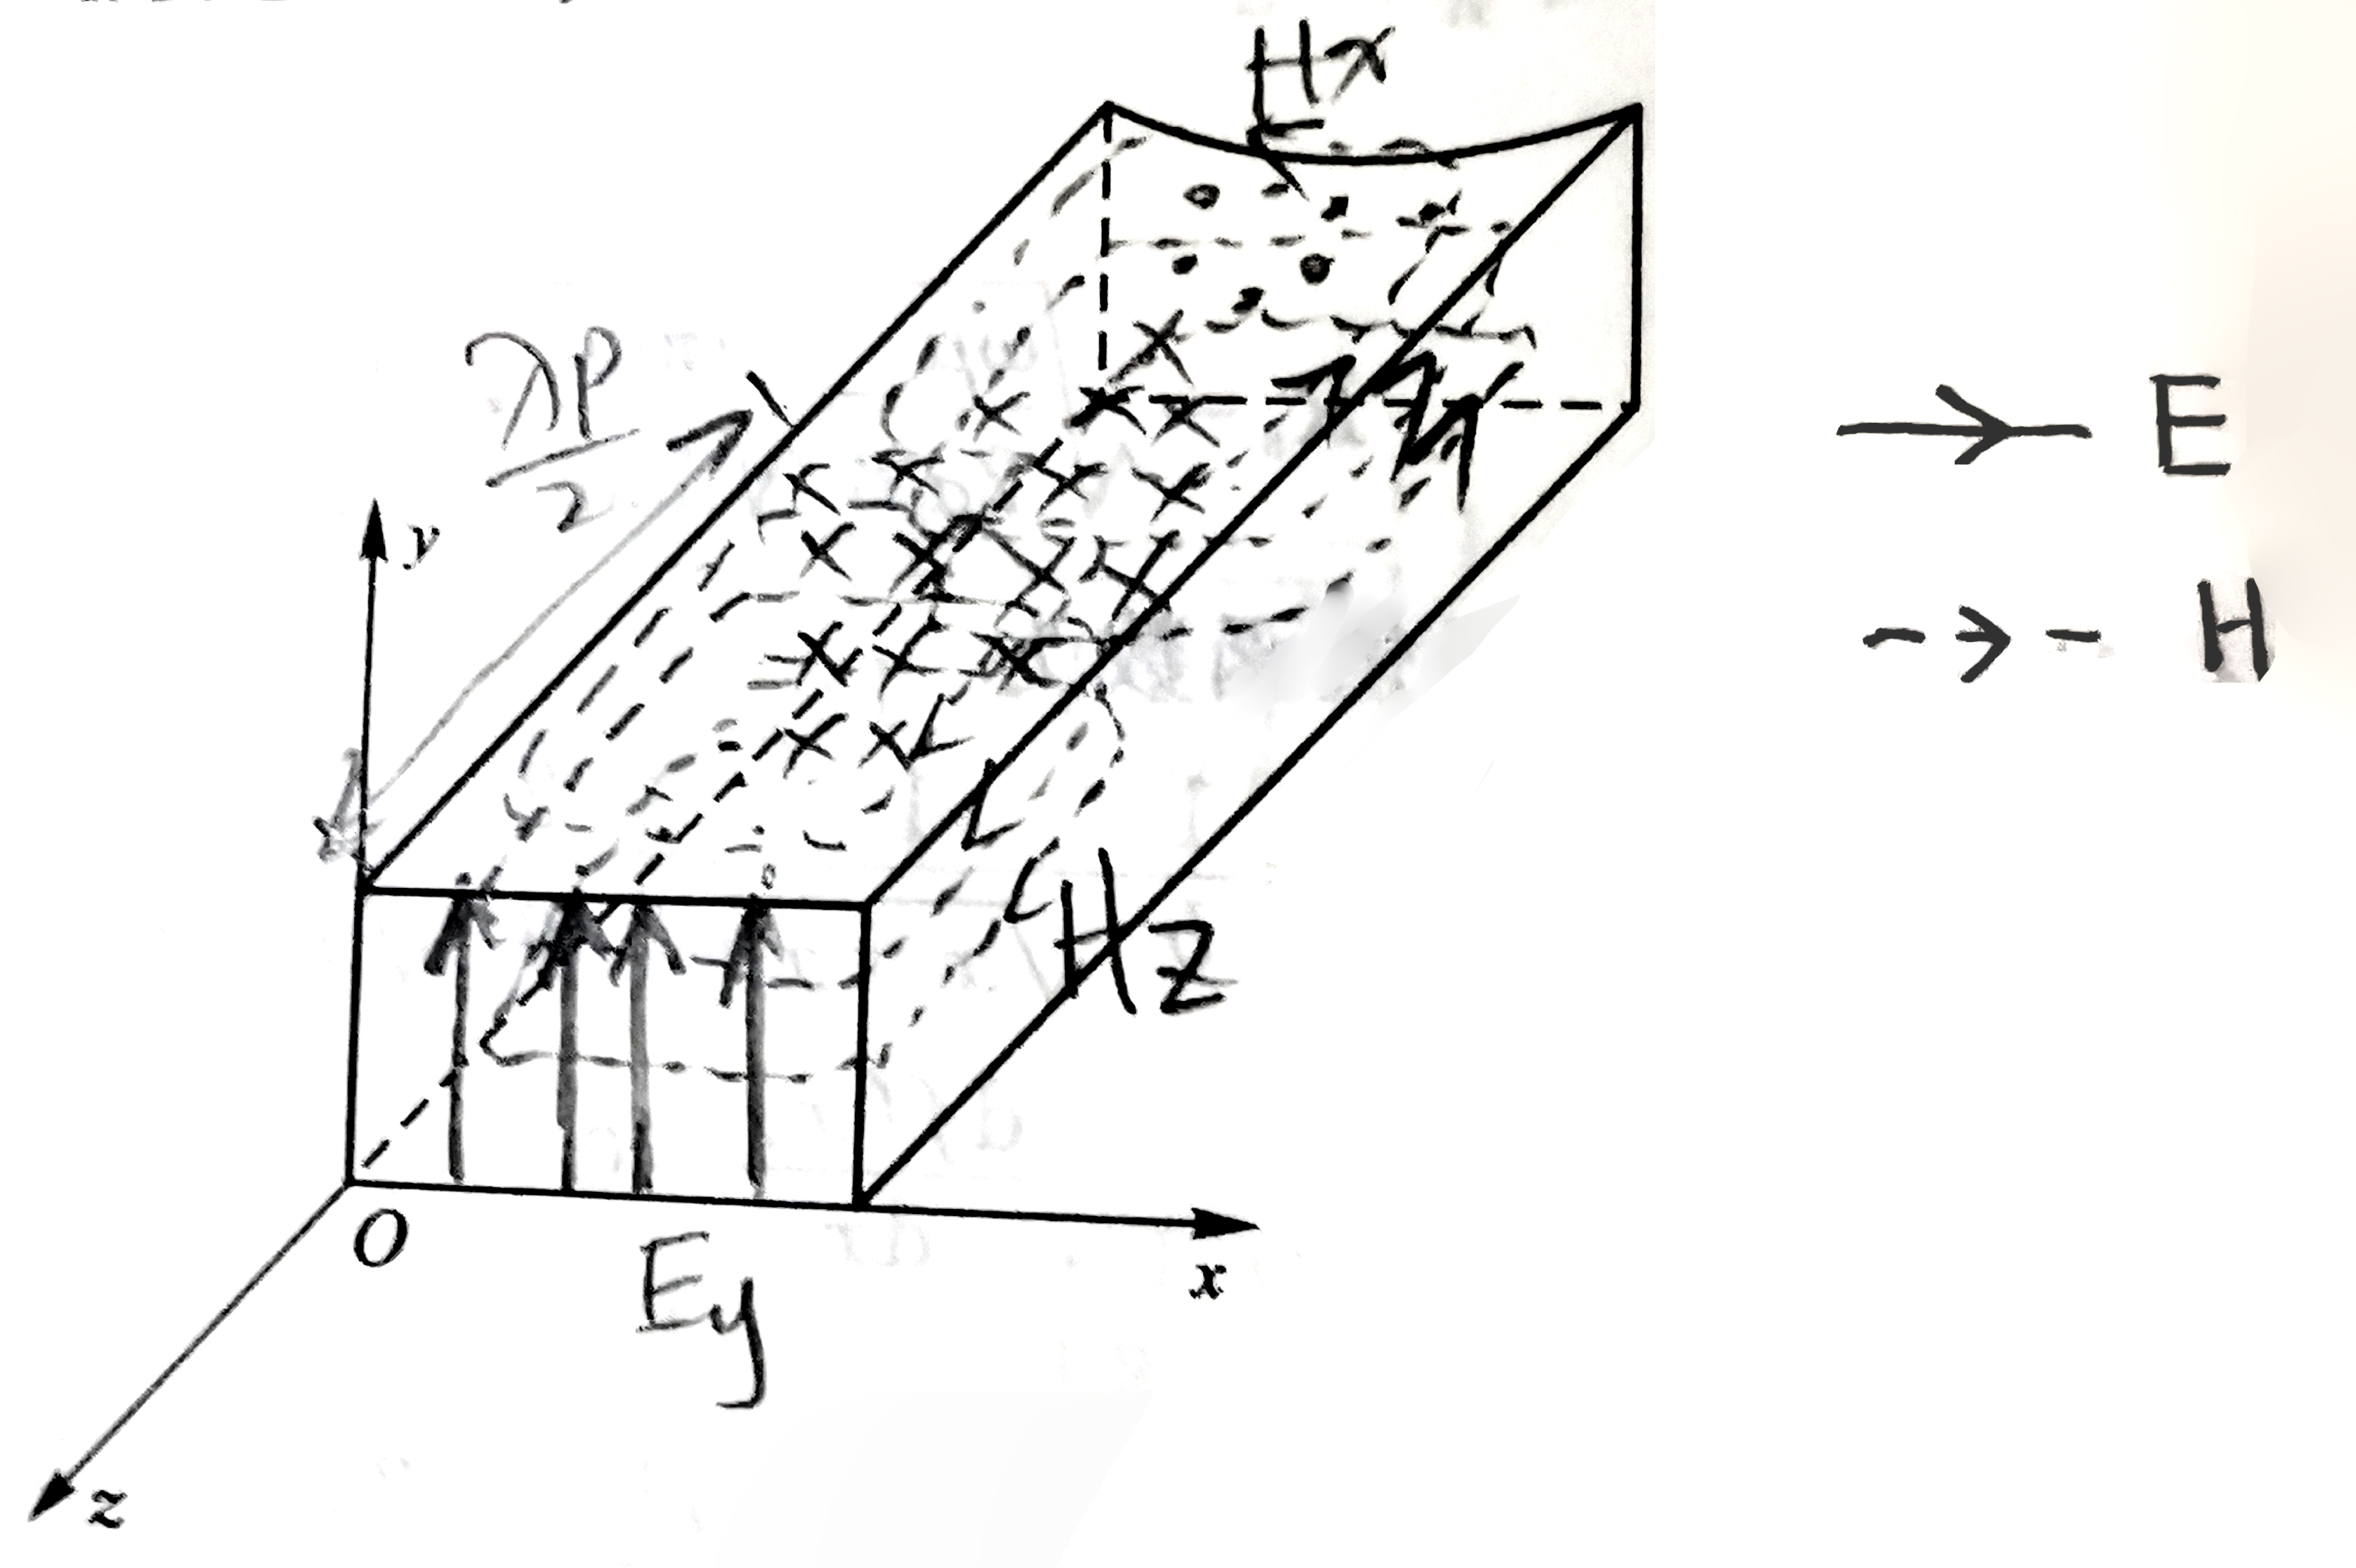
\includegraphics[width=10cm]{figure/appendix/2-3(2).jpg}
        \caption{\kaishu 2-3第二题图}\label{Fig: 2-3(2)}
    \end{figure}
    \paragraph{3}画出宽壁$y=0$的表面电流分布。指出何处$J_z$最大。
    \\{\bfseries 解:}如图\ref{Fig: 2-3(3)}所示。\\
    对于 TE{\scriptsize 10}模,宽壁内表面切向的磁场分量$H_s=H_x$,因此:
    \begin{equation*}
        J_z=\left[\hat{n}\times H_s\right]_{y=0}=\left[\hat{y}\times H_x\right]_{y=0}=-H_x|_{y=0}=\frac{\beta a}{\pi}H_0\sin\left(\frac{\pi}{a}x\right)\sin(\omega t-\beta z)
    \end{equation*}
    因此在$x=\frac{a}{2}$处取得最大值
    \begin{figure}[htp]
        \centering
        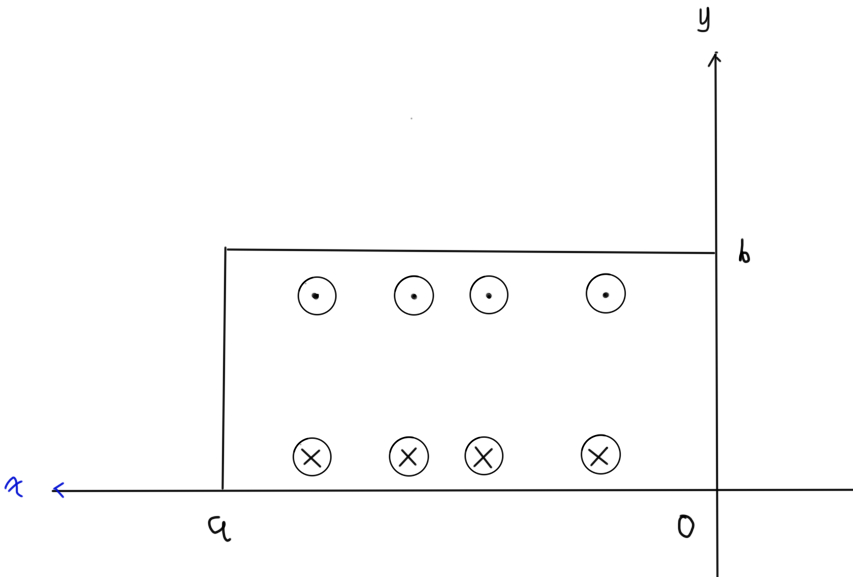
\includegraphics[width=8cm]{figure/appendix/2-3(3).jpg}
        \caption{\kaishu 2-3第三题图}\label{Fig: 2-3(3)}
    \end{figure}

\section{作业2-4}
    \paragraph{1}已知矩形波导如图\ref{Fig: 2-4(1)}所示,分别写出 TE{\scriptsize 11}模和 TM{\scriptsize 11}模的一般场方程。若要求它们是凋落模,写出条件。
    \begin{figure}[htp]
        \centering
        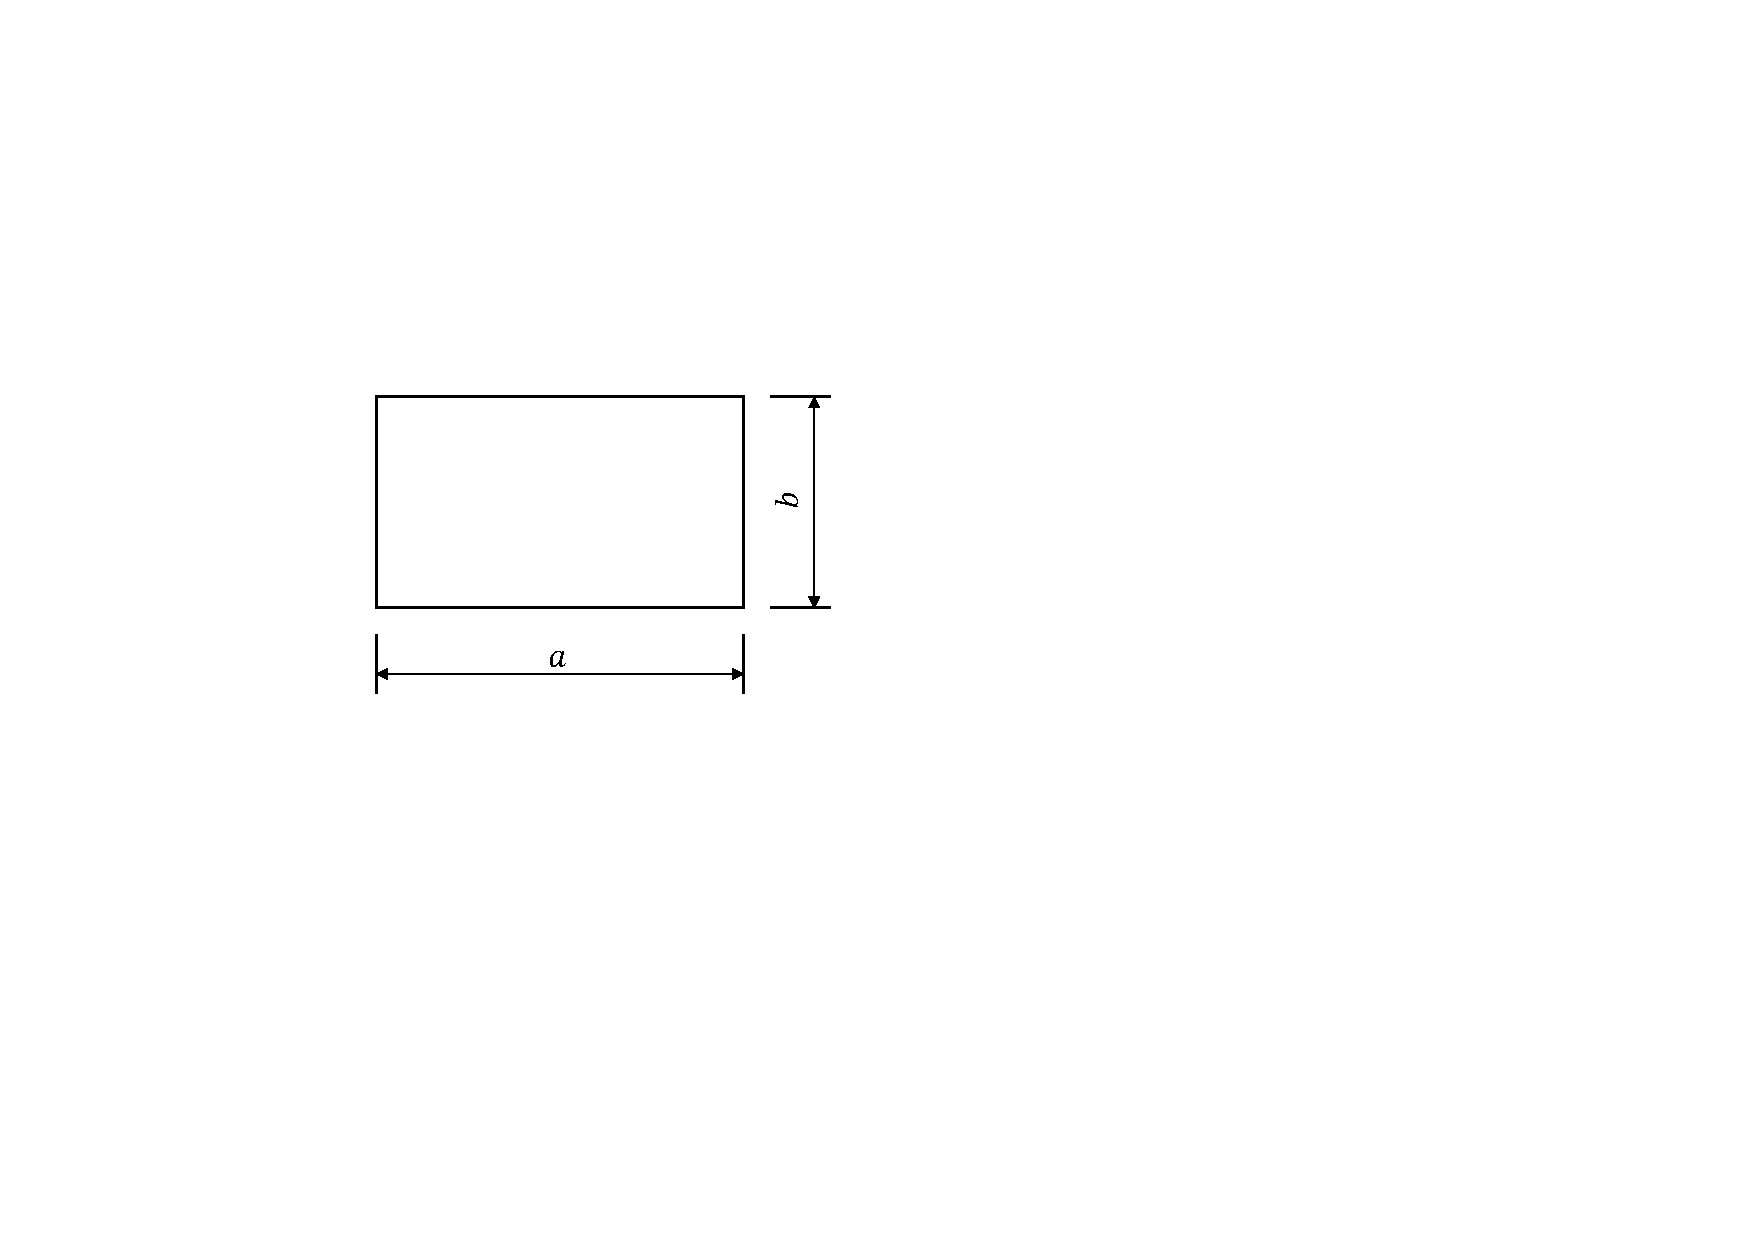
\includegraphics[width=6cm]{figure/appendix/2-4(1).pdf}
        \caption{\kaishu 2-4第一题图}\label{Fig: 2-4(1)}
    \end{figure}
    \\{\bfseries 解:}\\
    对于 TE{\scriptsize 11}模:
    \begin{subequations}
        \begin{numcases}{\mbox{TE{\scriptsize 11}纵向场}}
            E_z=0 \\
            H_z=H_0\cos{\left(\frac{\pi}{a}x\right)}\cos{\left(\frac{\pi}{b}y\right)}\mathrm{e}^{-\gamma z}
        \end{numcases}
    \end{subequations}
    其中$\gamma$满足$\gamma^2=k_c^2-k^2$,$k^2=\omega^2\mu \varepsilon$,$H_0$由激励决定。


    由纵向分量法,
    \begin{equation}
        \begin{bmatrix}
            E_x\\E_y\\H_x\\H_y
        \end{bmatrix}
        =\frac{1}{k_c^2}\begin{bmatrix}
            -\gamma&0&0&-\mathrm{j}\omega \mu\\
            0&-\gamma&\mathrm{j}\omega \mu&0\\
            0&\mathrm{j}\omega \varepsilon&-\gamma&0\\
            -\mathrm{j}\omega \varepsilon&0&0&-\gamma\\
        \end{bmatrix}
        \begin{bmatrix}
            \frac{\partial E_z}{\partial x}\\\frac{\partial E_z}{\partial y}\\\frac{\partial H_z}{\partial x}\\\frac{\partial H_z}{\partial y}
        \end{bmatrix}
    \end{equation}
    得:
    \begin{subequations}
        \begin{numcases}{\mbox{TE{\scriptsize 11}横向场}}
            E_x=\mathrm{j}\frac{\omega \mu}{k_c^2}\left(\frac{\pi}{b}\right)H_0\cos{\left(\frac{\pi}{a}x\right)}\sin{\left(\frac{\pi}{b}y\right)}\mathrm{e}^{-\gamma z}\\
            E_y=-\mathrm{j}\frac{\omega \mu}{k_c^2}\left(\frac{\pi}{a}\right)H_0\sin{\left(\frac{\pi}{a}x\right)}\cos{\left(\frac{\pi}{b}y\right)}\mathrm{e}^{-\gamma z}\\
            H_x=\frac{\gamma}{k_c^2}\left(\frac{\pi}{a}\right)H_0\sin{\left(\frac{\pi}{a}x\right)}\cos{\left(\frac{\pi}{b}y\right)}\mathrm{e}^{-\gamma z}\\
            H_y=\frac{\gamma}{k_c^2}\left(\frac{\pi}{b}\right)H_0\cos{\left(\frac{\pi}{a}x\right)}\sin{\left(\frac{\pi}{b}y\right)}\mathrm{e}^{-\gamma z}
        \end{numcases}
    \end{subequations}
    对于 TM{\scriptsize 11}模,将$E_z$分离变量$E_z=X(x)Y(y)$代入$\frac{\nabla^2_tE_z}{E_z}+k_c^2=0$,得
    \begin{equation}
        E_z=E_0\cos(k_xx+\varphi_x)\cos(k_yy+\varphi_y)\mathrm{e}^{-\gamma z}
    \end{equation}
    由纵向场法,
    \begin{subequations}
        \begin{numcases}{}
            E_x=E_0\frac{\gamma}{k_c^2}k_x\sin(k_xx+\varphi_x)\cos(k_yy+\varphi_y)\mathrm{e}^{-\gamma z} \\
            E_y=E_0\frac{\gamma}{k_c^2}k_y\cos(k_xx+\varphi_x)\sin(k_yy+\varphi_y)\mathrm{e}^{-\gamma z}
        \end{numcases}
    \end{subequations}
    将其代入矩形波导的边界条件
    \begin{subequations}
        \begin{numcases}{}
            E_y|_{x=0,a}=0 \\
            E_x|_{y=0,b}=0
        \end{numcases}
    \end{subequations}
    解得:
    \begin{subequations}
        \begin{numcases}{}
            k_x=\frac{m\pi}{x}\\
            k_y=\frac{n\pi}{b}\\
            \varphi_x=\frac{\pi}{2}\\
            \varphi_y=\frac{\pi}{2}
        \end{numcases}
    \end{subequations}
    其中$m=1,n=1$。因此得:
    \begin{subequations}
        \begin{numcases}{\mbox{TM{\scriptsize 11}纵向场}}
            E_z=E_0\sin{\left(\frac{\pi}{a}x\right)}\sin{\left(\frac{\pi}{b}y\right)}\mathrm{e}^{-\gamma z} \\
            H_z=0
        \end{numcases}
    \end{subequations}
    其中$\gamma$满足$\gamma^2=k_c^2-k^2$,$k^2=\omega^2\mu \varepsilon$,$E_0$由激励决定。


    同理由纵向场法,可以表示横向场:
    \begin{subequations}
        \begin{numcases}{\mbox{TM{\scriptsize 11}横向场}}
            E_x=-\frac{\gamma}{k_c^2}\left(\frac{\pi}{a}\right)E_0\cos{\left(\frac{\pi}{a}x\right)}\sin{\left(\frac{\pi}{b}y\right)}\mathrm{e}^{-\gamma z}\\
            E_y=-\frac{\gamma}{k_c^2}\left(\frac{\pi}{b}\right)E_0\sin{\left(\frac{\pi}{a}x\right)}\cos{\left(\frac{\pi}{b}y\right)}\mathrm{e}^{-\gamma z}\\
            H_x=\mathrm{j}\frac{\omega \varepsilon}{k_c^2}\left(\frac{\pi}{b}\right)E_0\sin{\left(\frac{\pi}{a}x\right)}\cos{\left(\frac{\pi}{b}y\right)}\mathrm{e}^{-\gamma z}\\
            H_y=-\mathrm{j}\frac{\omega \varepsilon}{k_c^2}\left(\frac{\pi}{a}\right)E_0\cos{\left(\frac{\pi}{a}x\right)}\sin{\left(\frac{\pi}{b}y\right)}\mathrm{e}^{-\gamma z}
        \end{numcases}
    \end{subequations}

    TE{\scriptsize 11}模和 TM{\scriptsize 11}模,其截止波长为
    \begin{equation*}
        \lambda_c=\frac{2}{\sqrt{\left(\frac{1}{a}\right)^2+\left(\frac{1}{b}\right)^2}}=\frac{2ab}{\sqrt{a^2+b^2}}
    \end{equation*}
    因此,当$\lambda>\frac{2ab}{\sqrt{a^2+b^2}}$时,TE{\scriptsize 11}模和 TM{\scriptsize 11}模为凋落模。
    \\[15pt]
    \paragraph{2}BJ-48波导工作在\SI{5}{\centi\metre}波段。$f\in[3.94\sim5.99]\si{\giga\hertz}$,$a\times b=47.55\times 22.15\,\si{\square\milli\metre}$,检验其是否符合波导设计标准。
    \\{\bfseries 解:}\\
    \begin{equation*}
        \lambda\in\left(\frac{c}{f_{max}},\frac{c}{f_{min}}\right)=\left(\SI{50.0835}{\milli\metre},\SI{76.1421}{\milli\metre}\right)
    \end{equation*}
    符合标准的波导参数$\hat{a},\hat{b}$,应满足:
    \begin{subequations}
        \begin{numcases}{}
            \mbox{功率容量尽量大:}\hat{a}>0.555 \lambda\\
            \mbox{TE{\scriptsize 10}传输条件:}2\hat{a}>\lambda\\
            \mbox{TE{\scriptsize 20}截止条件:}\hat{a}<\lambda\\
            \mbox{加宽频带}\frac{\hat{b}}{\hat{a}}<0.5
        \end{numcases}
    \end{subequations}
    因此:
    \begin{subequations}
        \begin{numcases}{}
            \hat{a}>0.555 \lambda_{max}=\SI{42.2589}{\milli\metre} \\
            \hat{a}<\lambda_{min}=\SI{50.0835}{\milli\metre}
        \end{numcases}
    \end{subequations}
    因此参数a满足条件。又
    \begin{equation*}
        \frac{b}{a}=\frac{22.15}{47.55}=0.4658<0.5
    \end{equation*}
    因此参数b也满足条件。

\section{作业2-6}
\begin{center}
\end{center}

    \paragraph{1}空气填充的圆波导内传输 TE{\scriptsize 01}模,已知$\frac{\lambda}{\lambda_c}=0.9$,$f=\SI{5}{\giga\hertz}$,求$\lambda_g$和$\beta$。若波导半径扩大一倍,$\beta$有何变化?
    \\{\bfseries 解:}\\
    TE{\scriptsize 01}模是圆波导中损耗最小的模,其截止波长为:
    \begin{equation*}
        \lambda_c=1.641R
    \end{equation*}
    电磁波波长
    \begin{equation*}
        \lambda=\frac{c}{f}=\frac{\SI{3e8}{\metre}}{\SI{5}{\giga\hertz}}=\SI{60}{\milli\metre}
    \end{equation*}
    因此,导波波长
    \begin{equation*}
        \lambda_g =\frac{\lambda}{\sqrt{1-\left(\frac{\lambda}{\lambda_c}\right)^2}}=\SI{137.65}{\milli\metre}
    \end{equation*}
    同时解得
    \begin{equation*}
        R=\frac{\lambda}{0.9\times 1.641}=\SI{40.63}{\milli\metre}
    \end{equation*}
    \begin{equation*}
        \beta=\frac{2\pi}{\lambda_g}=\SI{45.64}{\radian\per\metre}
    \end{equation*}
    当波导的半径扩大一倍,$\lambda_c$增大一倍,$\lambda_g $减小,$\beta$增大。
    \\[15pt]
    \paragraph{2}对工作频率为\SI{3}{\giga\hertz}的发射机,用矩形波导和圆波导馈电,均用主传输模,试比较尺寸的大小。
    \begin{equation*}
        \lambda=\frac{c}{f}=\frac{\SI{3e8}{\metre\per\second}}{\SI{3}{\giga\hertz}}=\SI{100}{\milli\metre}
    \end{equation*}
        传输 TE{\scriptsize 10}的矩形波导,有
        \begin{subequations}
            \begin{numcases}{}
                0.555 \lambda<a<\lambda \\
                \frac{\hat{b}}{a}<0.5
            \end{numcases}
        \end{subequations}
        因此$a_{max}=\lambda$,对应$b_{max}=0.5\lambda$。


        传输 TE{\scriptsize 11}模的圆形波导,有
        \begin{equation}
            \lambda_{c TM_{01}}<\lambda<\lambda_{c TE_{11}}
        \end{equation}
        即
        \begin{equation*}
            2.62R<\lambda<3.412R
        \end{equation*}
        因此
        \begin{equation*}
            R\in\left(\frac{\lambda}{3.412},\frac{\lambda}{2.62}\right)
        \end{equation*}
        综上,矩形波导尺寸最大为$ab=0.5 \lambda^2$,圆波导尺寸最大为$\pi R^2=\frac{\pi}{2.62^2}\lambda^2=0.4577\lambda^2$。
    \\[15pt]
    \paragraph{3}已知半径为R的圆波导,电场有唯一分量
    \begin{equation*}
        E_\phi=E_0 \mathrm{J}_1\left(\frac{3.832}{R}r\right)\mathrm{e}^{-\mathrm{j}\beta z}
    \end{equation*}
    \begin{enumerate}
        \renewcommand*\labelenumi{(\theenumi)} %设置enumerate标号为一对圆括号
        \item 它是TE还是TM模式?
        \item 求磁场$\vec{H}$;
        \item 分析它的模式指数$m,n$并说出其物理意义;
        \item 画出场型图。
    \end{enumerate}
    ~\\{\bfseries 解:}\\
    (1):由于电场没有纵向分量,因此为TE模式。\\
    (2):$\vec{H}=\frac{1}{-\mathrm{j}\omega\mu}\nabla\times\vec{E}$,在柱坐标系下:
    \begin{align}
        \vec{H}&=\frac{1}{-\mathrm{j}\omega\mu}\cdot\frac{1}{r}\begin{vmatrix}
            \hat{r}&r\hat{\phi}&\hat{z}\\
            \frac{\partial }{\partial r}&\frac{\partial }{\partial \phi}&\frac{\partial }{\partial z}\\
            E_r&rE_\phi&E_z
        \end{vmatrix}\\
        &=\frac{1}{-\mathrm{j}\omega\mu}\cdot\frac{1}{r}\begin{vmatrix}
            \hat{r}&r\hat{\phi}&\hat{z}\\
            \frac{\partial }{\partial r}&\frac{\partial }{\partial \phi}&\frac{\partial }{\partial z}\\
            0&rE_0 \mathrm{J}_1\left(\frac{3.832}{R}r\right)\mathrm{e}^{-\mathrm{j}\beta z}&0
        \end{vmatrix}\notag\\
        &=\frac{\mathrm{j}}{\omega\mu r}\left[\hat{r}\mathrm{j}\beta rE_0 \mathrm{J}_1\left(\frac{3.832}{R}r\right)\mathrm{e}^{-\mathrm{j}\beta z}+\hat{z}E_0 \mathrm{e}^{-\mathrm{j}\beta z}\frac{\partial r\mathrm{J}_1\left(\frac{3.832}{R}r\right)}{\partial r}\right]\notag
    \end{align}
    根据递推公式
    \begin{equation}
        x \mathrm{J}_m'\left(x\right)+m \mathrm{J}_m\left(x\right)=x \mathrm{J}_{m-1}\left(x\right)
    \end{equation}
    有
    \begin{equation}
        \frac{\mathrm{d}}{\mathrm{d}x} \left[x \mathrm{J}_1\left(x\right)\right]=x\mathrm{J}_0\left(x\right)
    \end{equation}
    因此,$\frac{\partial r\mathrm{J}_1\left(\frac{3.832}{R}r\right)}{\partial r}=\frac{\partial \left[(\frac{3.832}{R}r)\mathrm{J}_1\left(\frac{3.832}{R}r\right)\right]}{\partial (\frac{3.832}{R}r)}=\frac{3.832}{R}r\mathrm{J}_0\left(\frac{3.832}{R}r\right) $,
    \begin{equation*}
        \vec{H}=\frac{E_0}{\omega\mu}\mathrm{e}^{-\mathrm{j}\beta z}\left[-\hat{r}\beta \mathrm{J}_1\left(\frac{3.832}{R}r\right)+\hat{z}\frac{3.832}{R}\mathrm{J}_0\left(\frac{3.832}{R}r\right)\right]
    \end{equation*}
    (3): TE{\scriptsize 01}模。\\
    $m=0$,表示$\phi$方向上没有驻波,即$E_\phi,H_r$不随$\phi$改变。\\$n=1$,表示$r$方向上$E_\phi,H_r$有一个最大值。
    \begin{figure}[htp]
        \centering
        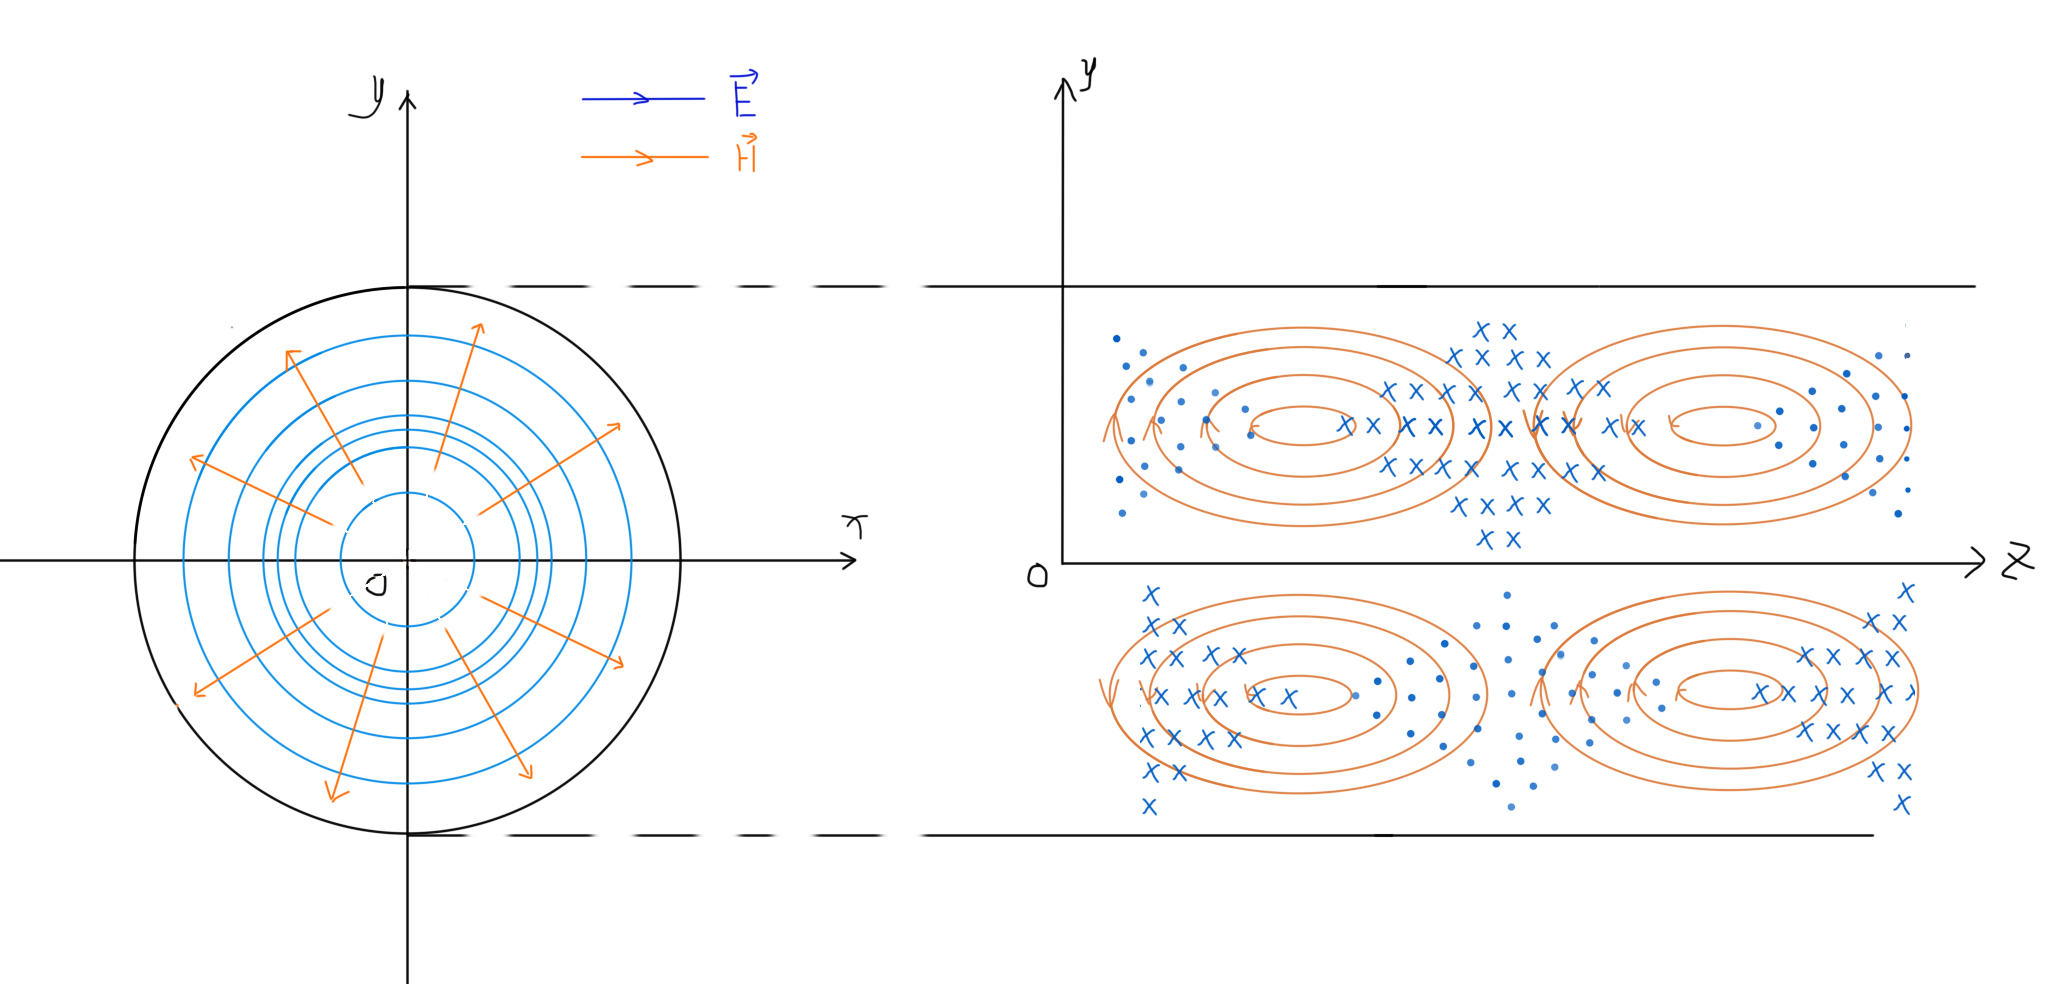
\includegraphics[width=15cm]{figure/appendix/2-6(3).jpg}
        \caption{\kaishu 2-6第三题图}\label{Fig: 2-6(3)}
    \end{figure}
    \\[15pt]
    \paragraph{4}已知半径为R的圆波导,磁场有唯一分量
    \begin{equation*}
        H_\phi=H_0 \mathrm{J}_0'\left(\frac{\nu_{01}}{R}r\right)\mathrm{e}^{-\mathrm{j}\beta z}
    \end{equation*}
    \begin{enumerate}
        \renewcommand*\labelenumi{(\theenumi)} %设置enumerate标号为一对圆括号
        \item 它是TE还是TM模式?
        \item 求磁场$\vec{E}$;
        \item 分析它的模式指数$m,n$并说出其物理意义;
        \item 画出场型图。
    \end{enumerate}
    ~\\{\bfseries 解:}\\
    (1):由于磁场没有纵向分量,因此为TM模式。\\
    (2):根据递推公式
    \begin{equation*}
        x \mathrm{J}_m'\left(x\right)+m \mathrm{J}_m\left(x\right)=x \mathrm{J}_{m-1}\left(x\right)
    \end{equation*}
    有
    \begin{equation*}
        \mathrm{J}_0'\left(x\right)=-\mathrm{J}_1\left(x\right)
    \end{equation*}
    因此,
    $\vec{E}=\frac{1}{\mathrm{j}\omega\varepsilon}\nabla\times\vec{H}$,在柱坐标系下:
    \begin{align}
        \vec{E}&=\frac{1}{\mathrm{j}\omega\varepsilon}\cdot\frac{1}{r}\begin{vmatrix}
            \hat{r}&r\hat{\phi}&\hat{z}\\
            \frac{\partial }{\partial r}&\frac{\partial }{\partial \phi}&\frac{\partial }{\partial z}\\
            H_r&rH_\phi&H_z
        \end{vmatrix}\\
        &=\frac{1}{\mathrm{j}\omega\varepsilon}\cdot\frac{1}{r}\begin{vmatrix}
            \hat{r}&r\hat{\phi}&\hat{z}\\
            \frac{\partial }{\partial r}&\frac{\partial }{\partial \phi}&\frac{\partial }{\partial z}\\
            0&rH_0 \mathrm{J}_0'\left(\frac{\nu_{01}}{R}r\right)\mathrm{e}^{-\mathrm{j}\beta z}&0
        \end{vmatrix}\notag\\
        &=\frac{1}{\mathrm{j}\omega\varepsilon r}\left[\hat{r}\mathrm{j}\beta rH_0 \mathrm{J}_0'\left(\frac{\nu_{01}}{R}r\right)\mathrm{e}^{-\mathrm{j}\beta z}+\hat{z}H_0 \mathrm{e}^{-\mathrm{j}\beta z}\frac{\partial r\mathrm{J}_0'\left(\frac{\nu_{01}}{R}r\right)}{\partial r}\right]\notag\\
        &=\frac{\mathrm{j}}{\omega\varepsilon r}\left[\hat{r}\mathrm{j}\beta rH_0 \mathrm{J}_1\left(\frac{\nu_{01}}{R}r\right)\mathrm{e}^{-\mathrm{j}\beta z}+\hat{z}H_0 \mathrm{e}^{-\mathrm{j}\beta z}\frac{\partial r\mathrm{J}_1\left(\frac{\nu_{01}}{R}r\right)}{\partial r}\right]\notag
    \end{align}

    代入$\frac{\partial r\mathrm{J}_1\left(\frac{\nu_{01}}{R}r\right)}{\partial r}=\frac{\partial\left[(\frac{\nu_{01}}{R}r)\mathrm{J}_1\left(\frac{\nu_{01}}{R}r\right)\right]}{\partial (\frac{\nu_{01}}{R}r)}=\frac{\nu_{01}}{R}r \mathrm{J}_0\left(\frac{\nu_{01}}{R}r\right)$,
    \begin{equation*}
        \vec{E}=\frac{H_0}{\omega\varepsilon}\mathrm{e}^{-\mathrm{j}\beta z}\left[-\hat{r}\beta \mathrm{J}_1\left(\frac{\nu_{01}}{R}r \right)+\hat{z}\frac{\nu_{01}}{R}\mathrm{J}_0\left(\frac{\nu_{01}}{R}r \right)\right]
    \end{equation*}
    (3): TM{\scriptsize 01}模。\\
    $m=0$,表示$\phi$方向上没有驻波,即$H_\phi,E_r$不随$\phi$改变。\\$n=1$,表示$r$方向上$E_\phi,H_r$有一个最大值。
    \begin{figure}[htp]
        \centering
        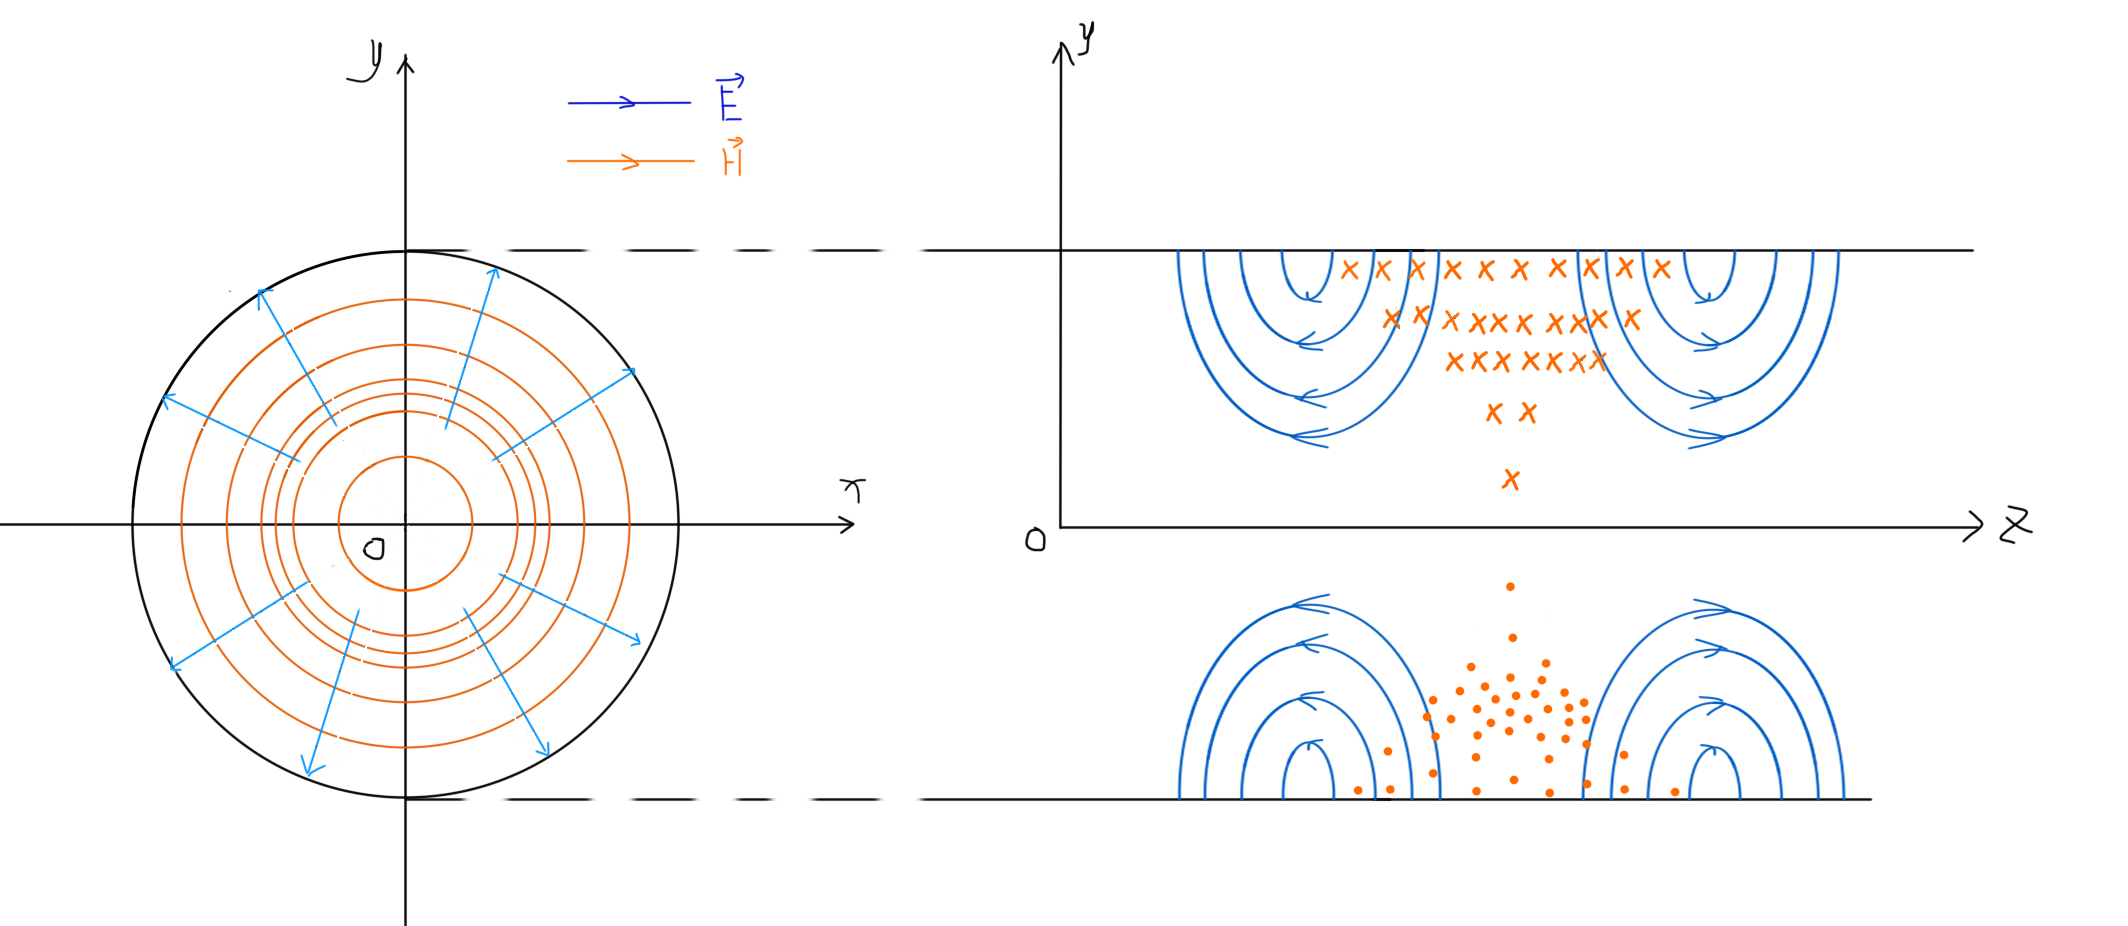
\includegraphics[width=15cm]{figure/appendix/2-6(4).jpg}
        \caption{\kaishu 2-6第四题图}\label{Fig: 2-6(4)}
    \end{figure}
    \\[15pt]
    \newpage
    \paragraph{5}横截面为半圆形波导,半径R。解出其中的 TE模和TM模。
    \\{\bfseries 解:}\\
    柱坐标下的亥姆霍兹方程:
    \begin{subequations}
        \begin{numcases}{}
            \nabla^2E_z+k^2E_z=0 \\
            \nabla^2H_z+k^2H_z=0
        \end{numcases}
    \end{subequations}
    其中
    \begin{equation}
        \nabla^2=\frac{1}{r}\frac{\partial }{\partial r}\left(r \frac{\partial }{\partial r}\right)+\frac{1}{r^2}\frac{\partial^2}{\partial \phi^2}+\frac{\partial^2}{\partial z^2}
    \end{equation}
    \begin{enumerate}
        \renewcommand*\labelenumi{\circled{\theenumi}}
        \item TE模:设
        \begin{equation}
            H_z=R(r)\varPhi(\phi)\mathrm{e}^{-\gamma z}\label{Equ: variables speration of Hz}
        \end{equation}
        展开亥姆霍兹方程,得
        \begin{equation}
            \frac{\partial^2H_z}{\partial r^2}+\frac{1}{r}\frac{\partial H_z}{\partial r}+\frac{1}{r^2}\frac{\partial^2H_z}{\partial \phi^2}+(\gamma^2+k^2)H_z=0\label{Equ: Helmholtz equation of Hz in cylindrical coordinate}
        \end{equation}
        令$\gamma^2+k^2=k_c^2$,并假设常数$m^2$,满足
        \begin{equation}
            \frac{1}{\varPhi}\frac{\mathrm{d}^2\varPhi}{\mathrm{d}\phi^2}=-m^2\label{Equ-Def: -m^2}
        \end{equation}
        代入式(\ref{Equ: variables speration of Hz})和式(\ref{Equ-Def: -m^2}),将方程(\ref{Equ: Helmholtz equation of Hz in cylindrical coordinate})整理为:
        \begin{equation}
            r^2 \frac{\mathrm{d}^2R}{\mathrm{d}r^2}+r \frac{\mathrm{d}R}{\mathrm{d}r}+(k_c^2r^2-m^2)R=0
        \end{equation}
        其通解为:
        \begin{subequations}
            \begin{numcases}{}
                \Phi(\phi)=c_1\cos m\phi+c_2\sin m\phi=\begin{pmatrix}
                    \cos m\phi\\\sin m\phi
                \end{pmatrix}\\
                R(r)=c_3 \mathrm{J}_m\left(k_cr\right)+c_4 \mathrm{N}_m\left(k_cr\right)=\begin{pmatrix}
                    \mathrm{J}_m\left(k_cr\right)\\\mathrm{N}_m\left(k_cr\right)
                \end{pmatrix}
            \end{numcases}
        \end{subequations}
        根据圆波导的特点和 Neumann 函数的性质,$R(r)$只应含有$c_3\mathrm{J}_m\left(k_cr\right)$项。因此:
        \begin{equation}
            H_z=H_0 \mathrm{J}_m\left(k_cr\right)\begin{pmatrix}
                    \cos m\phi\\\sin m\phi
                \end{pmatrix}\mathrm{e}^{-\gamma z}
        \end{equation}
        由纵向分量法,
        \begin{equation}
            \begin{bmatrix}
                E_r\\E_\phi\\H_r\\H_\phi
            \end{bmatrix}
            =\frac{1}{k_c^2}\begin{bmatrix}
                -\gamma&0&0&-\mathrm{j}\omega \mu\\
                0&-\gamma&\mathrm{j}\omega \mu&0\\
                0&\mathrm{j}\omega \varepsilon&-\gamma&0\\
                -\mathrm{j}\omega \varepsilon&0&0&-\gamma\\
            \end{bmatrix}
            \begin{bmatrix}
                \frac{\partial E_z}{\partial r}\\\frac{1}{r}\frac{\partial E_z}{\partial \phi}\\\frac{\partial H_z}{\partial r}\\\frac{1}{r}\frac{\partial H_z}{\partial \phi}
            \end{bmatrix}
        \end{equation}
        得(半)圆柱形波导TE模场的一般解:
        \begin{subequations}
            \begin{numcases}{}
                E_z=0 \\
                H_z=H_0 \mathrm{J}_m\left(k_cr\right)\begin{pmatrix}
                    \cos m\phi\\\sin m\phi
                \end{pmatrix}\mathrm{e}^{-\gamma z} \\
                E_r=\pm H_0\frac{\mathrm{j}\omega\mu m}{k_c^2r}\mathrm{J}_m\left(k_cr\right)\begin{pmatrix}
                    \sin m\phi\\\cos m\phi
                \end{pmatrix}\mathrm{e}^{-\gamma z} \\
                E_\phi=H_0\frac{\mathrm{j}\omega\mu}{k_c}\mathrm{J}_m'\left(k_cr\right)\begin{pmatrix}
                    \cos m\phi\\\sin m\phi
                \end{pmatrix}\mathrm{e}^{-\gamma z} \\
                H_r=-H_0\frac{\gamma}{k_c}\mathrm{J}_m'\left(k_cr\right)\begin{pmatrix}
                    \cos m\phi\\\sin m\phi
                \end{pmatrix}\mathrm{e}^{-\gamma z} \\
                H_\phi=\pm H_0\frac{\gamma m}{k_c^2r}\mathrm{J}_m\left(k_cr\right)\begin{pmatrix}
                    \sin m\phi\\\cos m\phi
                \end{pmatrix}\mathrm{e}^{-\gamma z}
            \end{numcases}\label{Equs: General Solution of TE Field in Half-cylinder}
        \end{subequations}\\
        由波导在$\phi$方向上的周期边界条件,可知$m\in\mathbb{Z}$;\\
        由半圆柱形波导的理想导体边界条件:
        \begin{subequations}
            \begin{numcases}{}
                E_r(\phi=0)=E_r(\phi=\pi)=0 \\
                E_\phi(r=R,0<\phi<\pi)=0
            \end{numcases}
        \end{subequations}
        代入式(\ref{Equs: General Solution of TE Field in Half-cylinder})中,得:
        \begin{subequations}
            \begin{numcases}{}
                H_0\frac{\mathrm{j}\omega\mu m}{k_c^2r}\mathrm{J}_m\left(k_cr\right)\begin{pmatrix}
                    0\\1
                \end{pmatrix}\mathrm{e}^{-\gamma z}=
                H_0\frac{\mathrm{j}\omega\mu m}{k_c^2r}\mathrm{J}_m\left(k_cr\right)\begin{pmatrix}
                    0\\\cos{m\pi}
                \end{pmatrix}\mathrm{e}^{-\gamma z}=0\label{Equ: TE boundary conditions NO.1 in Half-cylinder}\\
                H_0\frac{\mathrm{j}\omega\mu}{k_c}\mathrm{J}_m'\left(k_cR\right)\begin{pmatrix}
                    \cos m\phi\\\sin m\phi
                \end{pmatrix}\mathrm{e}^{-\gamma z}=0\label{Equ: TE boundary conditions NO.2 in Half-cylinder}
            \end{numcases}
        \end{subequations}
        由式(\ref{Equ: TE boundary conditions NO.2 in Half-cylinder}),可推知$\mathrm{J}_m'\left(k_cR\right)=0$,解得:
        \begin{equation}
            k_c=\frac{\mu_{mn}}{R}\,,\;n=1,2,\cdots
        \end{equation}
        其中$\mu_{mn}$为第一类$m$阶Bessel函数\underline{\bfseries 导数}的第$n$个根。\\
        式(\ref{Equ: TE boundary conditions NO.1 in Half-cylinder})中,由于$\mathrm{J}_m\left(k_cr\right)$仍可以取特定范围内的任意值,可推知待定系数$c_2=0$。\\
        因此,半圆柱形波导TE模场的解为
        \begin{subequations}
            \begin{numcases}{}
                E_z=0 \\
                H_z=H_0 \mathrm{J}_m\left(\frac{\mu_{mn}}{R}r\right)\cos (m\phi)\mathrm{e}^{-\gamma z} \\
                E_r=\pm H_0\frac{\mathrm{j}\omega\mu m}{k_c^2r}\mathrm{J}_m\left(\frac{\mu_{mn}}{R}r\right) \sin (m\phi)\mathrm{e}^{-\gamma z} \\
                E_\phi=H_0\frac{\mathrm{j}\omega\mu}{k_c}\mathrm{J}_m'\left(\frac{\mu_{mn}}{R}r\right)\cos (m\phi)\mathrm{e}^{-\gamma z} \\
                H_r=-H_0\frac{\gamma}{k_c}\mathrm{J}_m'\left(\frac{\mu_{mn}}{R}r\right)\cos (m\phi)\mathrm{e}^{-\gamma z} \\
                H_\phi=\pm H_0\frac{\gamma m}{k_c^2r}\mathrm{J}_m\left(\frac{\mu_{mn}}{R}r\right)\sin (m\phi)\mathrm{e}^{-\gamma z}
            \end{numcases}
        \end{subequations}
        ~\\[8pt]
        \item TM模:\\同理利用纵向场分量法,可以导出(半)圆柱形波导TM模场的一般解:
        \begin{subequations}
            \begin{numcases}{}
                E_z=E_0 \mathrm{J}_m\left(k_cr\right)\begin{pmatrix}
                    \cos m\phi\\\sin m\phi
                \end{pmatrix}\mathrm{e}^{-\gamma z} \\
                H_z=0\\
                E_r=-E_0\frac{\gamma}{k_c}\mathrm{J}_m'\left(k_cr\right)\begin{pmatrix}
                    \cos m\phi\\\sin m\phi
                \end{pmatrix}\mathrm{e}^{-\gamma z} \\
                E_\phi=\pm E_0\frac{\gamma m}{k_c^2r}\mathrm{J}_m\left(k_cr\right)\begin{pmatrix}
                    \sin m\phi\\\cos m\phi
                \end{pmatrix}\mathrm{e}^{-\gamma z} \\
                H_r=\mp E_0\frac{\mathrm{j}\omega\varepsilon m}{k_c^2r}\mathrm{J}_m\left(k_cr\right)\begin{pmatrix}
                    \sin m\phi\\\cos m\phi
                \end{pmatrix}\mathrm{e}^{-\gamma z} \\
                H_\phi=-E_0\frac{\mathrm{j}\omega\varepsilon}{k_c}\mathrm{J}_m'\left(k_cr\right)\begin{pmatrix}
                    \cos m\phi\\\sin m\phi
                \end{pmatrix}\mathrm{e}^{-\gamma z}
            \end{numcases}\label{Equs: General Solution of TM Field in Half-cylinder}
        \end{subequations}\\
        由波导在$\phi$方向上的周期边界条件,可知$m\in\mathbb{Z}$;\\
        由半圆柱形波导的理想导体边界条件:
        \begin{subequations}
            \begin{numcases}{}
                E_r(\phi=0)=E_r(\phi=\pi)=0 \\
                E_\phi(r=R,0<\phi<\pi)=0
            \end{numcases}
        \end{subequations}
        代入式(\ref{Equs: General Solution of TE Field in Half-cylinder})中,得:
        \begin{subequations}
            \begin{numcases}{}
                E_0\frac{\gamma}{k_c}\mathrm{J}_m'\left(k_cr\right)\begin{pmatrix}
                    1\\0
                \end{pmatrix}\mathrm{e}^{-\gamma z}=
                E_0\frac{\gamma}{k_c}\mathrm{J}_m'\left(k_cr\right)\begin{pmatrix}
                    \cos m\pi\\0
                \end{pmatrix}\mathrm{e}^{-\gamma z}=0\label{Equ: TM boundary conditions NO.1 in Half-cylinder}\\
                E_0\frac{\gamma m}{k_c^2R}\mathrm{J}_m\left(k_cR\right)\begin{pmatrix}
                    \sin m\phi\\\cos m\phi
                \end{pmatrix}\mathrm{e}^{-\gamma z}=0\label{Equ: TM boundary conditions NO.2 in Half-cylinder}
            \end{numcases}
        \end{subequations}
        由式(\ref{Equ: TE boundary conditions NO.2 in Half-cylinder}),可推知$\mathrm{J}_m\left(k_cR\right)=0$,解得:
        \begin{equation}
            k_c=\frac{\nu_{mn}}{R}\,,\;n=1,2,\cdots
        \end{equation}
        其中$\nu_{mn}$为第一类$m$阶Bessel函数的第$n$个根。\\
        式(\ref{Equ: TE boundary conditions NO.1 in Half-cylinder})中,由于$\mathrm{J}_m'\left(k_cr\right)$仍可以取特定范围内的任意值,可推知待定系数$c_1=0$。\\
        因此,半圆柱形波导TE模场的解为
        \begin{subequations}
            \begin{numcases}{}
                E_z=E_0 \mathrm{J}_m\left(\frac{\nu_{mn}}{R}r\right)\sin (m\phi) \mathrm{e}^{-\gamma z} \\
                H_z=0\\
                E_r=-E_0\frac{\gamma}{k_c}\mathrm{J}_m'\left(\frac{\nu_{mn}}{R}r\right)\sin (m\phi) \mathrm{e}^{-\gamma z} \\
                E_\phi=\pm E_0\frac{\gamma m}{k_c^2r}\mathrm{J}_m\left(\frac{\nu_{mn}}{R}r\right)\cos (m\phi)\mathrm{e}^{-\gamma z} \\
                H_r=\mp E_0\frac{\mathrm{j}\omega\varepsilon m}{k_c^2r}\mathrm{J}_m\left(\frac{\nu_{mn}}{R}r\right)\cos (m\phi)\mathrm{e}^{-\gamma z} \\
                H_\phi=-E_0\frac{\mathrm{j}\omega\varepsilon}{k_c}\mathrm{J}_m'\left(\frac{\nu_{mn}}{R}r\right)\sin (m\phi) \mathrm{e}^{-\gamma z}
            \end{numcases}
        \end{subequations}
    \end{enumerate}

    \section{作业2-7}
    \begin{center}
        姓名:韩玉千\hspace{4cm}学号:19020100423
    \end{center}

    \paragraph{1}论述TEM模传输线的主要特点,并说明它们满足什么支配方程。
    \\{\bfseries 解:}\\
        TEM传输线上,电场和磁场没有纵向分量:
        \begin{subequations}
            \begin{numcases}{\mbox{TEM模:}}
                \vec{E}_z=0 \\
                \vec{H}_z=0
            \end{numcases}
        \end{subequations}

    TEM模所满足的支配方程:\emph{Maxwell}方程组。

    \paragraph{2}导出圆同轴线的功率$P$和导体衰减常数$\alpha_c$的表达式。
    \\{\bfseries 解:}\\
    在圆同轴线中,电磁场分布:
    \begin{subequations}
        \begin{numcases}{}
            \vec{E}=\hat{r} E_0\frac{a}{r}\mathrm{e}^{-\mathrm{j}\beta z} \\
            \vec{H}=\hat{\varphi} \frac{E_0}{\eta}\frac{a}{r}\mathrm{e}^{-\mathrm{j}\beta z}
        \end{numcases}
    \end{subequations}
    同轴线内外导体间电压和内导体的轴向电流:
    \begin{subequations}
        \begin{numcases}{}
            U=\int_{a}^{b}E_r\,\mathrm{d}r=E_0a\ln\left(\frac{b}{a}\right)\mathrm{e}^{-\mathrm{j}\beta z} \\
            I=\left[\int_{0}^{2\pi}H_\varphi\,r\mathrm{d}\varphi\right]_{r=a}=\frac{2\pi E_0a}{\eta}\mathrm{e}^{-\mathrm{j}\beta z}
        \end{numcases}
    \end{subequations}
    平均坡印廷矢量:
    \begin{equation}
        \vec{S}_{av}=\Re\left[\frac{1}{2}\vec{E}\times \vec{H}^*\right]=\hat{z}\frac{E_0^2a^2}{2\eta r^2}
    \end{equation}
    因此,传输功率:
    \begin{equation}
        P=\int_{a}^{b}S_{av}\,2\pi r\mathrm{d}r=\frac{\sqrt{\varepsilon_r}}{120}E_0^2a^2\ln\left(\frac{b}{a}\right)
    \end{equation}
    衰减常数:
    \begin{equation}
        \alpha_c=\frac{8.686R_s\sqrt{\varepsilon_r}\left(1+\frac{b}{a}\right)}{2\pi b\left(120\ln\frac{b}{a}\right)}\qquad\si{\decibel\per\meter}
    \end{equation}

    \paragraph{3}研究如图所示的半填充圆同轴线。
    \begin{enumerate}
        \renewcommand*\labelenumi{(\theenumi)}
        \item 电场 $\vec{E}$和磁场 $\vec{H}$表达式。
        \item 传输波长$\lambda$。
        \item 波速$v_p$。
        \item 特性阻抗$Z_0$。
    \end{enumerate}
    \begin{figure}[htp]
        \centering
        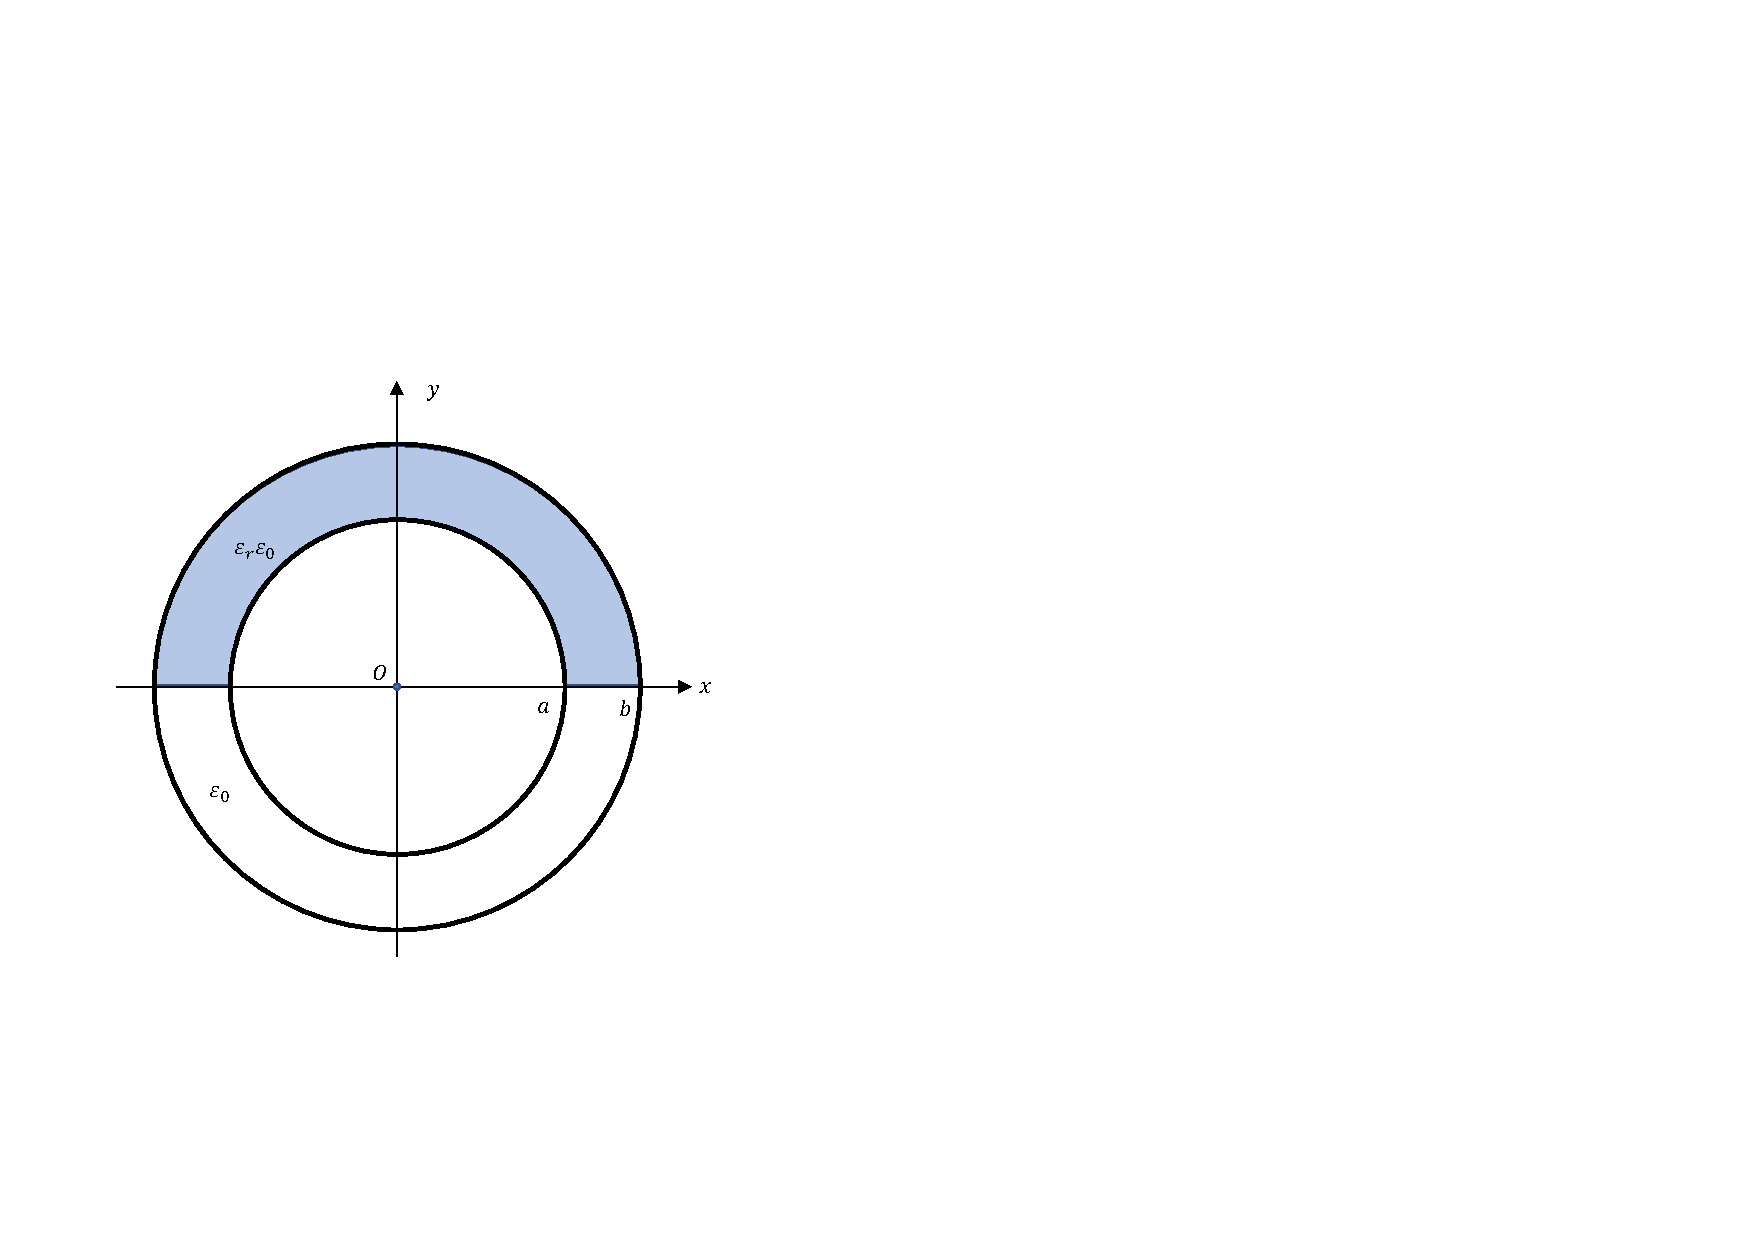
\includegraphics[width=6cm]{figure/appendix/2-7(3).pdf}
        \caption{\kaishu 2-7第三题图:半填充圆同轴线}\label{Fig: 2-7(3)}
    \end{figure}
    {\bfseries 解:}\\
    (1)



    \paragraph{4}有两种不同的圆同轴线$\dfrac{a_1}{b_1}=\dfrac{a_2}{b_2}$,$a_1>a_2$。
    \begin{figure}[htp]
        \centering
        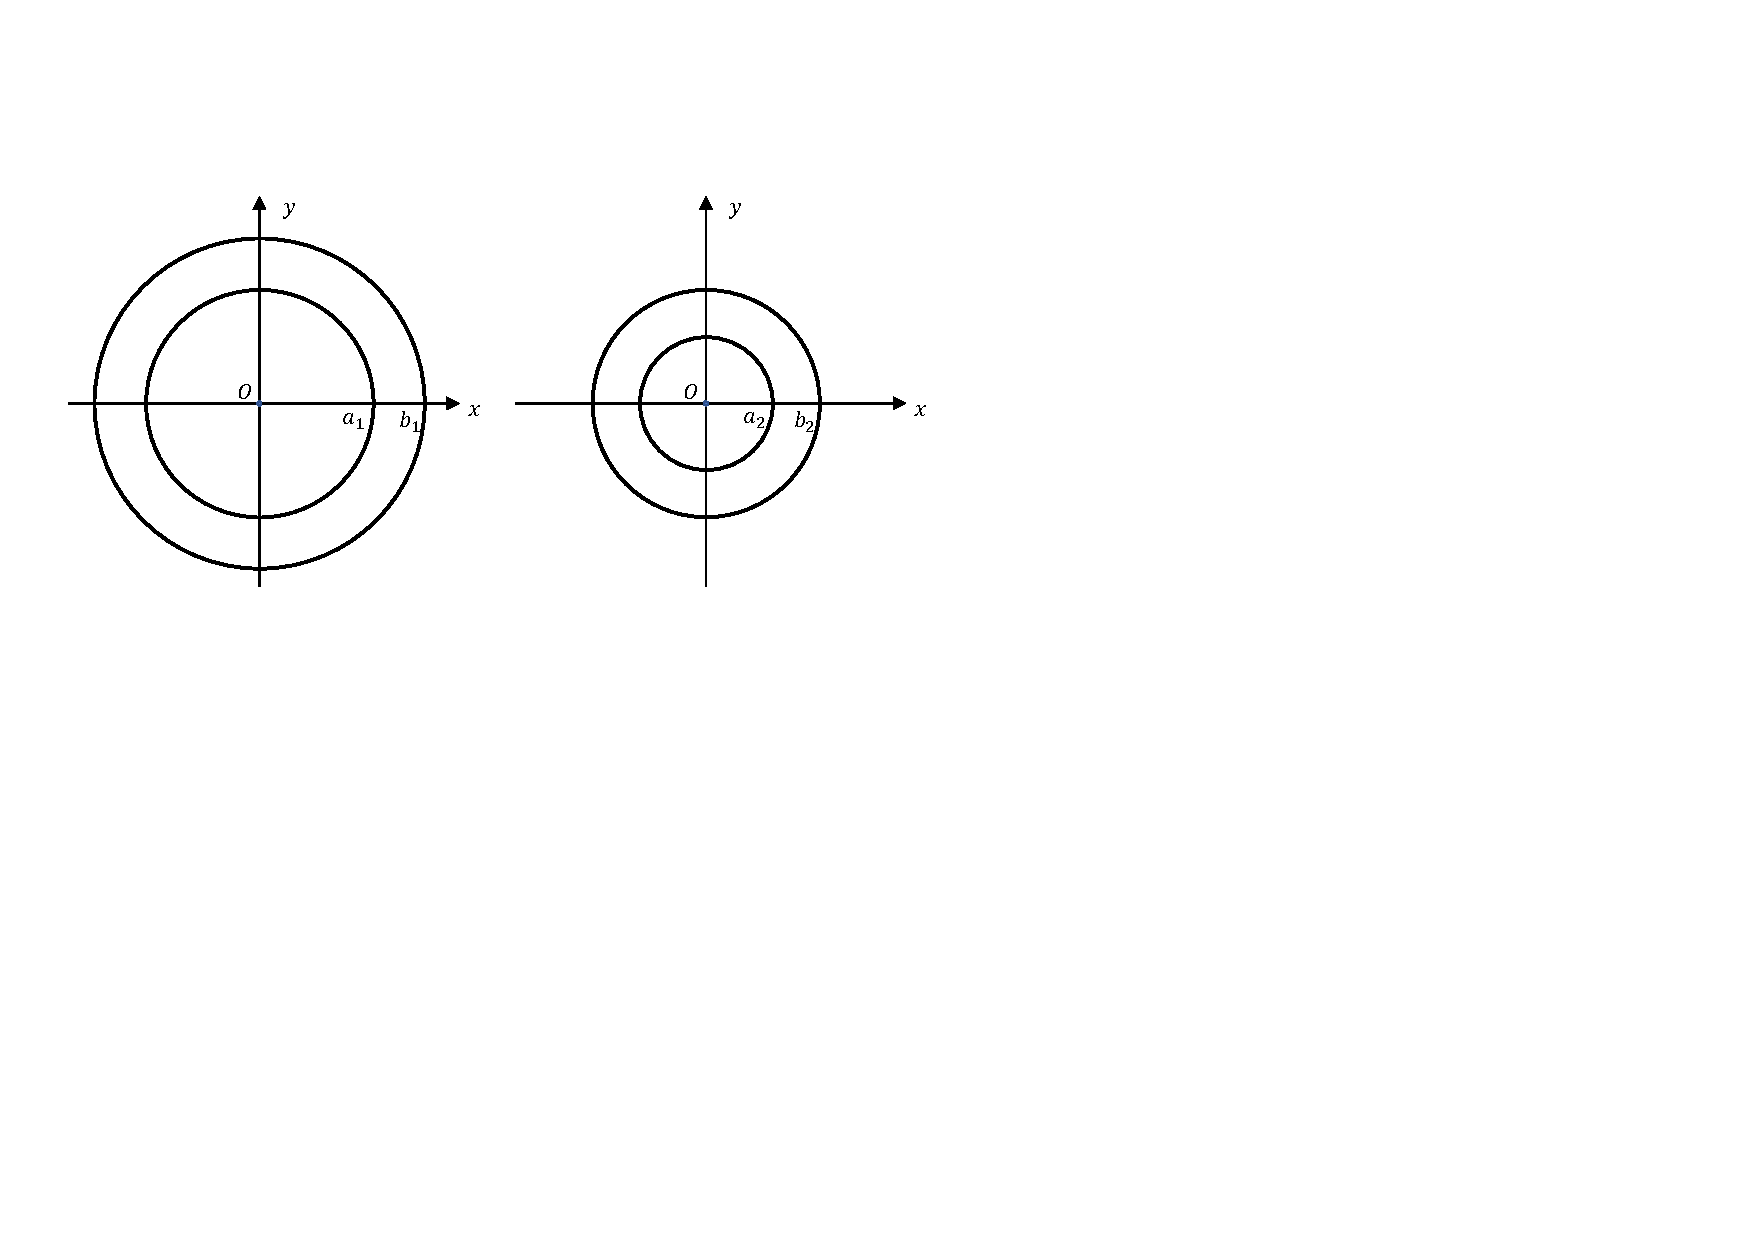
\includegraphics[width=12cm]{figure/appendix/2-7(4).pdf}
        \caption{\kaishu 2-7第四题图:两种圆同轴线}\label{Fig: 2-7(4)}
    \end{figure}
    \begin{enumerate}
        \renewcommand*\labelenumi{(\theenumi)}
        \item 哪种圆同轴线的特性阻抗$Z_0$大?
        \item 哪种圆同轴线的波长$\lambda$大?
        \item 哪种圆同轴线的功率容量$P_\mathrm{max}$大?
        \item 哪种圆同轴线的TEM模频带宽?
    \end{enumerate}
    {\bfseries 解:}\\
    (1)


    \paragraph{5}圆同轴线如下图。采用$\nabla_t^2 \vec{E}=0$和$\nabla_t^2 \vec{H}=0$求其TEM主模。已知圆对称,即$\frac{\partial }{\partial \varphi}=0$,且$\vec{E}=\hat{r}E$,$\vec{H}=\hat{\varphi}H$。

    \begin{figure}[htp]
        \centering
        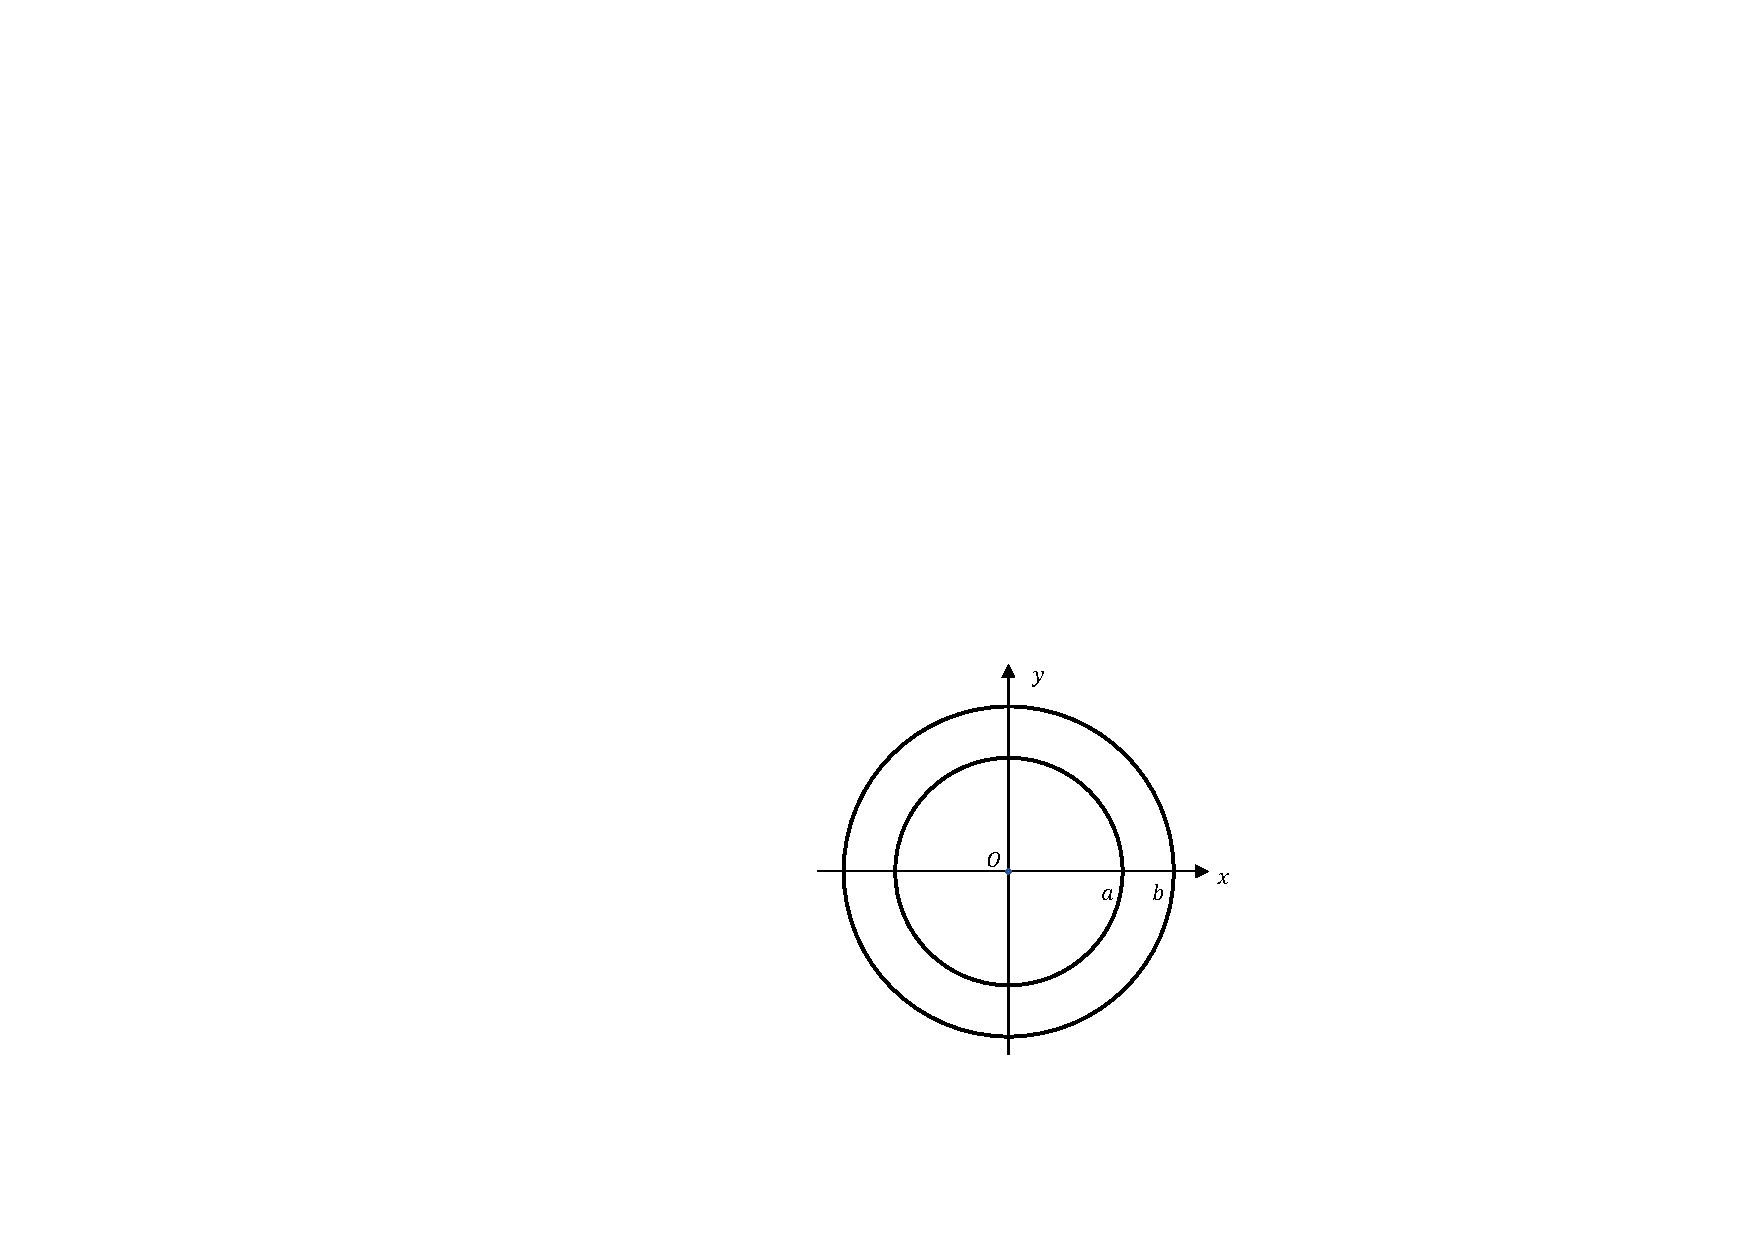
\includegraphics[width=6cm]{figure/appendix/2-7(5).pdf}
        \caption{\kaishu 2-7第五题图:圆同轴线}\label{Fig: 2-7(5)}
    \end{figure}

    {\bfseries 解:}\\
